\begin{frame}
\frametitle{5.6 (August 2016)}
\begin{block}{OTB}
\begin{itemize}
\item Parallélisation de l'exécution du pipeline avec la librairie MPI
\item Extraction et sélection d'échantillons pour la classification supervisée
\item Amélioration de la classification données vecteurs
\item Support des images Sentinel-1 (calibration géométrique)
\end{itemize}
\end{block}

\begin{block}{Monteverdi 3.4}
\begin{itemize}
\item Amélioration affichage et accès aux OTB applications
\end{itemize}
\end{block}
\end{frame}

\begin{frame}[fragile]
\frametitle{Parallélisation de traitements OTB avec MPI}
\begin{center}
  \vspace{-0.5cm}
  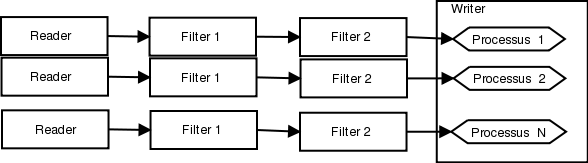
\includegraphics[width=0.6\textwidth]{images/mpi.png}
  \begin{scriptsize}
\begin{verbatim}
    $ mpirun -np $nb_procs --hostfile $PBS_NODEFILE  \
    otbcli_BundleToPerfectSensor \
    -inp $ROOT/IMG_PHR1A_P_001/IMG_PHR1A_P_201605260427149_ORT_1792732101-001_R1C1.JP2 \
    -inxs $ROOT/IMG_PHR1A_MS_002/IMG_PHR1A_MS_201605260427149_ORT_1792732101-002_R1C1.JP2 \
    -out $ROOT/pxs.tif uint16 -ram 1024

    ------------ JOB INFO 1043196.tu-adm01 -------------
    
    JOBID           : 1043196.tu-adm01
    USER            : michelj
    GROUP           : ctsiap
    JOB NAME        : OTB_mpi
    SESSION         : 631249
    RES REQSTED     : mem=1575000mb,ncpus=560,place=free,walltime=04:00:00
    RES USED        : cpupercent=1553,cput=00:56:12,mem=4784872kb,ncpus=560,vmem=18558416kb,
    walltime=00:04:35
    BILLING         : 42:46:40 (ncpus x walltime)
    QUEUE           : t72h
    ACCOUNT         : null
    JOB EXIT CODE   : 0
    
    ------------ END JOB INFO 1043196.tu-adm01 ---------
\end{verbatim}
\end{scriptsize}
\end{center}
\end{frame}
